\section{Introduction}

The idea of using trapped ions for quantum computing has been around for a long time~\cite{Shore1993,Meekhof1996} but one of the most promising turned out to be the architecture proposed by Molmer and Sorenson in 1999~\cite{MolmerSorenson} which then began to be achieved experimentally soon after~\cite{Wineland2000,Monroe2000}.

One of the problems turned out, however, to be heating during the operation of the gate~\cite{Berkeland1998,HAFFNER2008,Johnson2016}.  The ability of the gate to perform universal quantum computation depends on the system's vibrational quantum number staying reasonably constant.  Much work looked at possible mechanisms for observed heating including r.f. heating~\cite{Turchette2000} and micromotion.

The basic Hamiltonian is, as laid out by Molmer and Sorenson~\cite{MolmerSorenson}.
\begin{align*}
  \hat{H} &= \hat{H}_0 + \hat{H}_{\text{int}} \\
  \hat{H}_0 &= \hbar \nu \left(  \hat{a}^{\dagger} \hat{a}   + \frac{1}{2}\right)  + \frac{\hbar \omega_{eg}}{2} \sum_{i} \sigma_{zi} \\
  \hat{H}_{\text{int}} &= \sum_{i} \frac{\hbar \Omega_i}{2} \left( \sigma_{+i} e^{i \left[ \eta_i \left( \hat{a}^{\dagger} + \hat{a} \right) - \omega_i t \right]}  +  \sigma_{-i} e^{-i \left[ \eta_i \left( \hat{a}^{\dagger} + \hat{a} \right) - \omega_i t \right]} \right)
\end{align*}
To which we will focus on $\hat{H}_{\text{int}}$.  The form supplied in these equations makes the tacit assumption that the transition strength is constant with respect to the nuclear configuration of the system; the only nuclear component of the transition comes from the recoil operator($e^{-i  \eta_i \left( \hat{a}^{\dagger} + \hat{a} \right) }$) coming from the laser momentum projected onto the direction of the trap.  Put another way, the actual Rabi frequency $\Omega_i$ approximately does not change with vibrational state.  Condon first articulated this approximation~\cite{Condon} for molecular spectra in 1928 but recent scholarship has shown lots of ways this approximation can lead to incorrect interpretation of experiments involving electronic transitions~\cite{MavrosNonCondon,hellerGraphene,photosyntheticKappa}. In particular, because (if one thinks of things in the position basis) a transition dipole variation such as this will deform the wavefunction upon application, this does imply that the system is heated upon laser excitation if this is indeed the case.  Since Heating is a constant problem for the operation of any quantum computer, we take it upon ourselves to investigate the effect a variation in transition dipole will have on a Molmer-Sorenson type System.


Mathematically, this means we are taking $\Omega_i$ and adding a position dependence which can then be decomposed into creation and annihilation operators
\begin{align}
	\Omega_i &\rightarrow \Omega_i \mu(x) \\
	\mu(x) &= \mu_0 \sum_{i=0} \kappa^{(i)} x^i \\
	&= \mu_0 \sum_{i=0} c^{(i)} \left( \hat{a} + \hat{a}^{\dagger}\right)^i
\end{align}
We assume that $c^{(1)}=0$ and all odd numbered corrections because the excited vibrational manifold is no different than the excited vibrational manifold so only symmetric orders in $x$ should physically be present.  Furthermore, and linear dependence would directly effect the calculated Rabi Frequency $\tilde{\Omega}$ but we are looking for an insipid effect to explain heating, not a major effect that should have been noticed by now.

We then explore a rather drastic shift and set $c^{(2)} = .1$ and explore the effect it would have on the dynamics of the system.  To wit, we recreate Figure 2 in ~\cite{MolmerSorenson} with this system in our Figure \ref{fig:c2_big_dynamics}.  This is a very large effect which would doubtless make a system completely unusable.


\begin{figure}
   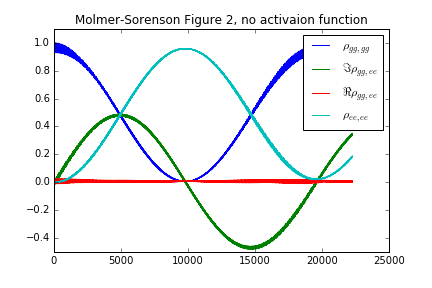
\includegraphics[width=1.0\columnwidth]{MS_fig2_noAct.png}
   \caption{This is a reproduction of Figure 2 from the original paper by Molmer and Sorenson where they proposed using a gate which operates like this to perform quantum computations.  Any needed state is accessible by turning off the excitation lasers at a given time during operation.}
	\label{fig:MS_big_dynamics}
\end{figure}


\begin{figure}
   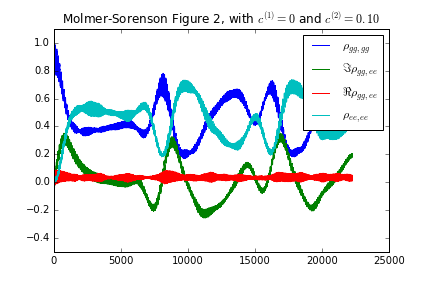
\includegraphics[width=1.0\columnwidth]{MS_fig2_c2.png}
   \caption{This is what Figure 2 from the original paper by Molmer and Sorenson would have looked like with a large quadratic term in the transition dipole $\mu(x)$.  Note that the nice unitary dynamics are almost completely gone.  This is not due, however, to heating but tot he}
	\label{fig:c2_big_dynamics}
\end{figure}



We next look at the Fidelity~\cite{Bowdrey2002} of the state compared to the ideal, unitary dynamics for multiple values of $c^{(2)}$ from $10^{-5}\rightarrow 1$ and plot the result in Figure \ref{fig:c2_fidelity deviation}.  As would be expected, small corrections don't induce much of a problem at all, but larger correction have the potential to affect the fidelity a great deal.
\begin{figure}
   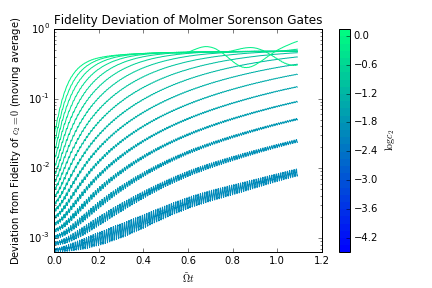
\includegraphics[width=1.0\columnwidth]{MS_fidelityDeviation_cComparison.png}
   \caption{ This show on a log scale the deviation from the ideal unitary dynamics for various values of  $c^{(2)}$.  Notably, the larger the value of  $c^{(2)}$, the greater the deviation.  The effect is still not very big.}
	\label{fig:c2_fidelity deviation}
\end{figure}

Another way of looking at this would be the average quantum number of the gate during operation and we plot that for the same values of  $c^{(2)}$ in Figure \ref{fig:MS_heating_cComparison}.  The laser beam appears to impart some heat at the beginning based on the value of $c^{(2)}$ but the value is not much.  What is increasing is the variation in the expected quantum number.  If we calculate, instead, the standard deviation of the vibrational quantum number, there is a clear trend up as $c^{(2)}$ goes up as seen in Figure \ref{fig:MS_heating_stdev}

\begin{figure}
   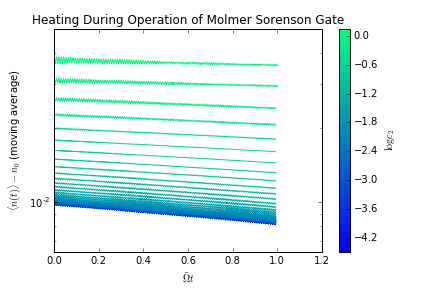
\includegraphics[width=1.0\columnwidth]{MS_heating_cComparison.png}
   \caption{ This show on a log scale the expected value of the vibrational quantum number during gate operation, for various values of  $c^{(2)}$.  Once again, the larger the value of  $c^{(2)}$, the greater the amount of heating but oddly, compared to such effects in ultrafast systems, the system very quickly reaches the higher level of heat, and then very slowly declines as the laser continues operation.  This effect is also not terribly large}
	\label{fig:MS_heating_cComparison}
\end{figure}


\begin{figure}
   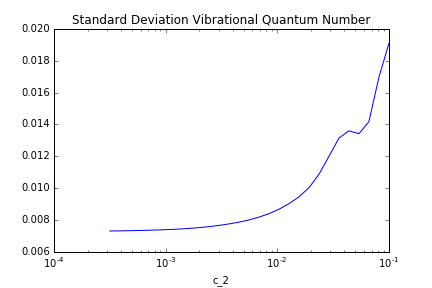
\includegraphics[width=1.0\columnwidth]{stdev_heating.png}
   \caption{ This show on a linear scale the standard deviation of the vibrational quantum number during gate operation, for various values of  $c^{(2)}$.  There is a very clear increasing relationship between this variation and  $c^{(2)}$.  This increases uncertainty in the state of the gate when the laser is turned off. }
	\label{fig:MS_heating_stdev}
\end{figure}


\section{Typical values for $c^{(i)}$}
If we take Yb+, and do a back of the envelope calculation.  The

\section{Conclusion}
We have shown the effect that a term quadratic in the nuclear position on the transition operator, can do to the fidelity of a Molmer-Sorenson gate.  Values of this term are, however, likely not large enough to be of any concern to experimentalists as they are very small.  As trap frequencies get higher and traps begin to include more and more atoms, this effect could potentially cascade and cause problems for future implementations of trapped-ion quantum computers.


\section{Supplemental Material}

\subsection{Rabi Frequency}

We want to see how this will nuclear dependence of the transition dipole will affect the calculated Rabi Frequency (to second order).  The formula in the original paper is

\begin{align*}
	\left(  \frac{\tilde{\Omega}}{2} \right)^2 &= \frac{1}{\hbar^2} \left|  \sum_m  \frac{\bra{een}H_{\text{int}}  \ket{m}\bra{m} H_{\text{int}} \ket{ggn} }{E_{ggn} + \hbar \omega_i - E_m} \right|^2
\end{align*}
Our $H_{\text{int}}$ for this derivation will assume $\eta = \eta_i = \eta_2$ and $\Omega = \Omega_1 = \Omega_2$ and has the added vibrational transition dipole moment $f(z)$
\begin{align*}
	\hat{H}_{\text{int}} &= \frac{\hbar \Omega}{2} \sum_{i}  \left( f(z) \sigma_{+i} e^{i \left[ \eta\left( \hat{a}^{\dagger} + \hat{a} \right) - \omega_i t \right]}  + f^*(z) \sigma_{-i} e^{-i \left[ \eta \left( \hat{a}^{\dagger} + \hat{a} \right) - \omega_i t \right]} \right)
\end{align*}
now we act this on the appropriate states:

\begin{align*}
	\hat{H}_{\text{int}} \ket{ggn} &= \frac{\hbar \Omega}{2}f(z) e^{i \eta\left( \hat{a}^{\dagger} + \hat{a} \right) } \left(  \ket{egn}e^{- i\omega_1 t } + \ket{gen}e^{- i\omega_2 t }   \right) \\
	\hat{H}_{\text{int}} \ket{een} &= \frac{\hbar \Omega}{2}f^*(z) e^{-i \eta\left( \hat{a}^{\dagger} + \hat{a} \right) } \left(  \ket{egn}e^{ i\omega_2 t } + \ket{gen}e^{i\omega_1 t }   \right)
\end{align*}
if we do as the paper does and restrict $m$ to be $\ket{egn+1}, \ket{gen-1}$

\begin{align*}
	\bra{gen - 1}\hat{H}_{\text{int}} \ket{ggn} &= \frac{\hbar \Omega}{2}\bra{gen - 1}f(z) e^{i \eta\left( \hat{a}^{\dagger} + \hat{a} \right) } \left(  \ket{egn}e^{- i\omega_1 t } + \ket{gen}e^{- i\omega_2 t }   \right) \\
	&= \frac{\hbar \Omega}{2}  \bra{n-1} f(z) e^{i \eta\left( \hat{a}^{\dagger} + \hat{a} \right) } \ket{n}e^{- i\omega_2 t }   \\
	\bra{egn + 1}\hat{H}_{\text{int}} \ket{ggn} &= \frac{\hbar \Omega}{2}\bra{egn + 1}f(z) e^{i \eta\left( \hat{a}^{\dagger} + \hat{a} \right) } \left(  \ket{egn}e^{- i\omega_1 t } + \ket{gen}e^{- i\omega_2 t }   \right) \\
	&= \frac{\hbar \Omega}{2}\bra{n + 1}f(z) e^{i \eta\left( \hat{a}^{\dagger} + \hat{a} \right) } \ket{n}e^{- i\omega_1 t }
\end{align*}
then the de-excitations from the doubly excited state
\begin{align*}
	\bra{gen - 1}\hat{H}_{\text{int}} \ket{een} &= \frac{\hbar \Omega}{2}\bra{gen - 1} f^*(z) e^{-i \eta\left( \hat{a}^{\dagger} + \hat{a} \right) } \left(  \ket{egn}e^{ i\omega_2 t } + \ket{gen}e^{i\omega_1t }   \right)\\
	&= \frac{\hbar \Omega}{2}\bra{n - 1} f^*(z) e^{-i \eta\left( \hat{a}^{\dagger} + \hat{a} \right) } \ket{n}e^{i\omega_1 t }   \\
	\bra{egn + 1}\hat{H}_{\text{int}} \ket{een} &= \frac{\hbar \Omega}{2}\bra{egn + 1} f^*(z) e^{-i \eta\left( \hat{a}^{\dagger} + \hat{a} \right) } \left(  \ket{egn}e^{ i\omega_2 t } + \ket{gen}e^{i\omega_1 t }   \right)\\
	&= \frac{\hbar \Omega}{2}\bra{n + 1} f^*(z) e^{-i \eta\left( \hat{a}^{\dagger} + \hat{a} \right) }  \ket{n}e^{ i\omega_2 t }
\end{align*}

Now is the time to think.  Our vibrational correction to the electronic transition moment, should only have even corrections to it.  And Molmer and Sorenson only expanded the laser recoil operator out to first order, meaning a typical matrix element from above will look like:
\begin{align*}
	\bra{n + 1} f^*(z) e^{-i \eta\left( \hat{a}^{\dagger} + \hat{a} \right) }  \ket{n} &\approx -i \eta \bra{n + 1} f^*(z) \left( \hat{a}^{\dagger} + \hat{a} \right)  \ket{n}
\end{align*}
and since $f$ will look like this:
\begin{align*}
	 f(z) &= 1 + c^{(2)}\left( \hat{a}^{\dagger} + \hat{a}  \right)^2 \\
	 &= 1 + c^{(2)}\left( \hat{a}^{\dagger}\hat{a}^{\dagger} + \hat{a}\hat{a}^{\dagger} + \hat{a}^{\dagger}\hat{a} + \hat{a}\hat{a}  \right)
\end{align*}
quick math aside:
\begin{align*}
	 [\hat{a}, \hat{a}^{\dagger}] &= 1\\
	 \hat{a} \hat{a}^{\dagger} - \hat{a}^{\dagger}\hat{a} &= 1\\
	 \hat{a} \hat{a}^{\dagger} - \hat{N} &= 1\\
	 \hat{a} \hat{a}^{\dagger}  &= 1 + \hat{N}
\end{align*}
\begin{align*}
	 f(z) &= 1 + c^{(2)}\left( \hat{a}^{\dagger}\hat{a}^{\dagger} + \left(  1 + \hat{N} \right) + \hat{N} + \hat{a}\hat{a}  \right) \\
	 &= 1 + c^{(2)}  + 2 c^{(2)} \hat{N} +  c^{(2)}\left( \hat{a}^{\dagger}\hat{a}^{\dagger} + \hat{a}\hat{a}  \right)
\end{align*}
So this indicates that we must be very careful when adding an $f(z)$ term as we're trying to imply an effect that hasn't been seen before, so we ought to renormalize and keep the Rabi Frequency the same as what we saw before we knew there was a polynomial transition dipole.
\begin{align*}
	 f(z) &= 1 - c^{(2)} (1 + 2 \bar{n}_0 ) + c^{(2)}\left( \hat{a}^{\dagger} + \hat{a}  \right)^2
\end{align*}

\subsection{Proper Unitary Dynamics}
According to Molmer and Sorenson's original paper, when you input both detunings to both ions, you get the following dynamics which are essentially a quantum process matrix... after a little bit of algebra
\begin{align*}
	\ket{gg} &\rightarrow \cos \left(\frac{\tilde{\Omega} T}{2} \right) \ket{gg} + i  \sin \left(\frac{\tilde{\Omega} T}{2} \right)\ket{ee}\\
	\ket{ee} &\rightarrow \cos \left(\frac{\tilde{\Omega} T}{2} \right) \ket{ee} + i  \sin \left(\frac{\tilde{\Omega} T}{2} \right) \ket{gg}\\
	\ket{ge} &\rightarrow \cos \left(\frac{\tilde{\Omega} T}{2} \right) \ket{ge} - i  \sin \left(\frac{\tilde{\Omega} T}{2} \right) \ket{eg}\\
	\ket{eg} &\rightarrow \cos \left(\frac{\tilde{\Omega} T}{2} \right) \ket{eg} - i  \sin \left(\frac{\tilde{\Omega} T}{2} \right) \ket{ge}
\end{align*}
If we want to know what the density matrix elements are, this requires some more work:
being a bit more mathematically precise we get:
\begin{align*}
	U(T)\ket{gg} &= \cos \left(\frac{\tilde{\Omega} T}{2} \right) \ket{gg} + i  \sin \left(\frac{\tilde{\Omega} T}{2} \right)\ket{ee}\\
	U(T)\ket{ee} &= \cos \left(\frac{\tilde{\Omega} T}{2} \right) \ket{ee} + i  \sin \left(\frac{\tilde{\Omega} T}{2} \right) \ket{gg}\\
	U(T)\ket{ge} &= \cos \left(\frac{\tilde{\Omega} T}{2} \right) \ket{ge} - i  \sin \left(\frac{\tilde{\Omega} T}{2} \right) \ket{eg}\\
	U(T)\ket{eg} &= \cos \left(\frac{\tilde{\Omega} T}{2} \right) \ket{eg} - i  \sin \left(\frac{\tilde{\Omega} T}{2} \right) \ket{ge}
\end{align*}
which will give us the elements of $U(T)$,
\begin{align*}
	\bra{gg}U(T)\ket{gg} &= \cos \left(\frac{\tilde{\Omega} T}{2} \right) \\
	\bra{ee}U(T)\ket{gg} &=  i  \sin \left(\frac{\tilde{\Omega} T}{2} \right)\\
	\bra{ee}U(T)\ket{ee} &= \cos \left(\frac{\tilde{\Omega} T}{2} \right) \\
	\bra{gg}U(T)\ket{ee} &=  i  \sin \left(\frac{\tilde{\Omega} T}{2} \right) \\
	\bra{ge}U(T)\ket{ge} &= \cos \left(\frac{\tilde{\Omega} T}{2} \right) \\
	\bra{eg}U(T)\ket{ge} &= - i  \sin \left(\frac{\tilde{\Omega} T}{2} \right)\\
	\bra{eg}U(T)\ket{eg} &= \cos \left(\frac{\tilde{\Omega} T}{2} \right) \\
	\bra{ge}U(T)\ket{eg} &=  - i  \sin \left(\frac{\tilde{\Omega} T}{2} \right)
\end{align*}
so there are all the nonzero elements of the time-evolution operator.
\begin{align*}
	U(T) &= \begin{bmatrix}
		\cos \left(\frac{\tilde{\Omega} T}{2} \right) & 0 & 0 & i\sin \left(\frac{\tilde{\Omega} T}{2} \right) \\
		0 & \cos \left(\frac{\tilde{\Omega} T}{2} \right) & -i\sin \left(\frac{\tilde{\Omega} T}{2} \right) & 0\\
		0 & -i\sin \left(\frac{\tilde{\Omega} T}{2} \right)  & \cos \left(\frac{\tilde{\Omega} T}{2} \right) & 0\\
		i\sin \left(\frac{\tilde{\Omega} T}{2} \right)  & 0 & 0 & \cos \left(\frac{\tilde{\Omega} T}{2} \right) \\
	\end{bmatrix}
\end{align*}
You can see from above that $U^{\dagger}U = I$ as we would expect
And we can use this operator to calculate the time-dependent density matrix through:
\begin{align*}
	\rho(T) &= \ket{\Psi(T)}\bra{\Psi(T)} \\
	&= U(T) \ket{\Psi(0)}\bra{\Psi(0)} U^{\dagger}(T)\\
	&= U(T) \rho(0) U^{\dagger}(T)
\end{align*}
